%!TEX root = practicum2.tex
\section{Results}

\subsection{Probability}

\begin{figure}[h!]
	\centering
	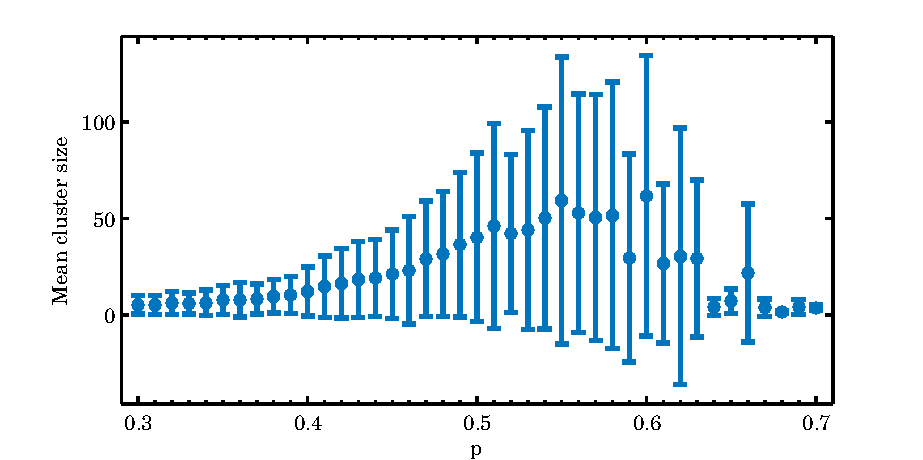
\includegraphics[width=\textwidth]{./img/assignment_a_mean_std_p.pdf}
	\caption{Mean cluster sizes, represented as points, and standard deviations, indicated by the vertical error bars, as a function of $p$, with a step size of $0.1$. The mean and standard deviation were calculated over $200$ runs on a $41 \times 41$ grid.}
	\label{fig:experiment:prob:mean_std_clusters}
\end{figure}

\subsection{System Size}

\begin{figure}[h!]
	\centering
	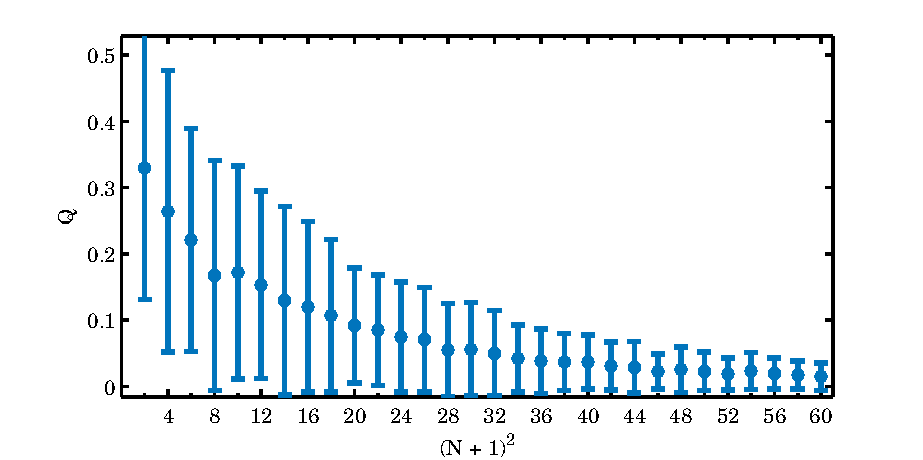
\includegraphics[width=\textwidth]{./img/assignment_b_mean_std_n.pdf}
	\caption{The mean, represented as points, and standard deviations, indicated by the error bars, of the ratio of the cluster size to number of sites in the grid, i.e. $(N + 1)^2$.The mean and standard deviation were calculated over $200$ runs with $p = 0.5$.}
	\label{fig:experiment:size:mean_std_clusters}
\end{figure}

\subsection{Connectivity}

\begin{figure}[h!]
	\centering
	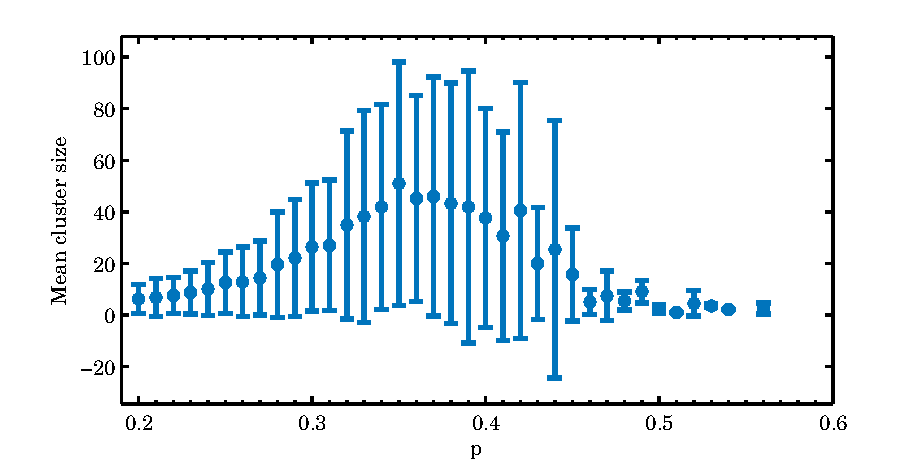
\includegraphics[width=\textwidth]{./img/assignment_d_mean_std_p.pdf}
	\caption{Mean cluster sizes, represented as points, and standard deviations, indicated by the vertical error bars, as a function of $p = 0.2, 0.21, \dotsc, 0.6$ when eight-connectivity is used. The mean and standard deviation were calculated over $200$ runs on a $41 \times 41$ grid.}
	\label{fig:experiment:conn:mean_std_clusters}
\end{figure}